\begin{title}
  Поверхность в пространстве $R^3$
\end{title}

\begin{define}
  $\vec \varphi = (x(u, \upsilon) , y(u, \upsilon), z(u, \upsilon)) ~~~
  (u, \upsilon) \in [D]$ непрерывно дифференцируема
  $$
  \rang \left(
  \begin{array}{ccc}
    x'_u & y'_u & y'_u \\
    x'_{\upsilon} & y'_{\upsilon} & y'_{\upsilon}
  \end{array}
  \right) = 2 ~~~
  \text{тогда называют поверхность гладкой}
  $$
  $[D] \leftrightarrow P \subset R^3$ то образ $\vec \varphi([D]) = P$
  называется простой поверхностью в $R^3$ а отображение
  $\vec \varphi(u, \upsilon)$ еe параметрическим заданием.
\end{define}

\begin{define}[эквивалентности поверхностей]
  $\vec \rho = \vec \rho(p,s) \sim \vec \varphi(u, \upsilon) ~~~
  (\rho, s) \in [\Omega]$ если возможна замена параметра
  $$
  \left\{
  \begin{array}{l}
    u = u(p,s) \\
    \upsilon = \upsilon(p,s)
  \end{array}
  \right. ~~~ [\Omega] \leftrightarrow [D] ~~~
  \left|
  \begin{array}{cc}
    \upsilon'_p & \upsilon'_s \\
    v'_p & v'_s
  \end{array}
  \right| \not = 0
  $$
  тогда $\vec \rho = \vec \rho(p,s) = \vec \varphi (x(u(p,s), \upsilon(p,s)),
  y(u(p,s), \upsilon(p,s)), z(u(p,s), \upsilon(p,s)))$

  $\vec \varphi ([D]) = P = \vec \rho([\Omega])$
\end{define}

\begin{define}[почти простой поверхности]
  $\vec \rho(u, \upsilon)$ гладкое отображение которое отображается
  взаимооднозначно в область $D$
  (может быть не ограничена) на какое-то множество в $R^3$, если $\exists$
  исчерпание $[D_n]$ такое что $P_n = \vec \varphi ([D_n])$
  является простой тогда $\vec P =
  \varphi(D)$ называется почти простой.
\end{define}

\begin{theorem}
  $P$ простая поверхность заданная парасетрически $(u, \upsilon) \in [D]$
  $\vec \varphi (u, \upsilon) = (x(u, \upsilon), y(u, \upsilon),
  z(u, \upsilon))$ тогда $d\vec \varphi = \vec \varphi'_udu +
  \vec \varphi'_{\upsilon} d\upsilon$
\end{theorem}

\begin{proof}
  $$
  [\vec \varphi_u, \vec \varphi_{\upsilon}] \not = \vec 0 =
  \left|
  \begin{array}{ccc}
    \vec i & \vec j & \vec k \\
    x'_u & y'_u & z'_u \\
    x'_{\upsilon} & y'_{\upsilon} & z'_{\upsilon}
  \end{array}
  \right| =
  $$
  $$
  = \vec i \left|
  \begin{array}{cc}
    y'_u & z'_u \\
    y'_{\upsilon} & z'_{\upsilon}
  \end{array}
  \right| +
  \vec j \left|
  \begin{array}{cc}
    z'_u & x'_u \\
    z'_{\upsilon} & x'_{\upsilon}
  \end{array}
  \right| +
  \vec k \left|
  \begin{array}{cc}
    x'_u & y'_u \\
    x'_{\upsilon} & u'_{\upsilon}
  \end{array}
  \right| \not = 0
  $$
  так как $\rang(...) = 2$ и будет хотябы один определитель не нулевой
\end{proof}

\begin{theorem}
  $\vec \varphi(u, \upsilon) \sim \vec \rho(p,s) ~~~ (p, s) \in [\Omega]$ тогда
  $[\vec \rho'_p, \vec \rho'_s]$ либо соноправлены либо противоположенно
  направленны.

  При замене параметризации меняется направления векторов.
\end{theorem}

\begin{proof}
  $\vec \rho(p,s) = \vec \varphi(u(p,s), \upsilon(p,s))$
  $$
  [\vec \rho'_p, \vec \rho'_s] = [\vec \varphi'_u u'_p +
  \vec \varphi'_{\upsilon} \upsilon'_p, \vec \varphi'_u u'_s +
  \vec \varphi'_{\upsilon} \upsilon'_s] =
  $$
  $$
  = [\vec \varphi'_u, \vec \varphi'_{\upsilon}] (u'_p \upsilon'_s -
  u'_s \upsilon'_p) = [\vec \varphi'_u, \vec \varphi'_{\upsilon}]
  \left|
  \begin{array}{cc}
    u'_p & u'_s \\
    \upsilon'_p & \upsilon'_s
  \end{array}
  \right| = 0
  $$
\end{proof}

\begin{define}
  $$
  \frac{d \vec \varphi}{dt} ~~ \text{касательный вектор}
  $$
  $$
  \frac{d \vec \varphi}{dt} \perp [\vec \varphi'_u, \vec \varphi'_{\upsilon}]
  = \vec n
  $$
  Векто нормали это вектор перпендикулярен всем прямым проходящим через точку
  $t$

  Поверхности бывают одностороними и двусторонними.

  Меры обладают свойством конечной адитивности то есть если разделить что-то
  на конечное кол-во частей то сумма всех мер будет равна мере всей части.
\end{define}

\begin{define}[первой квадратичной формы]
  $$
  \vec \varphi' = \vec \varphi_u u' + \vec \varphi_{\upsilon} \upsilon'
  $$
  $$
  |\vec \varphi'|^2 = (\vec \varphi', \vec \varphi') =
  (\vec \varphi_u u' + \vec \varphi_{\upsilon} \upsilon', \vec \varphi_u u' +
  \vec \varphi_{\upsilon} \upsilon') =
  $$
  $$
  = (\vec \varphi_u, \vec \varphi_u)u'^2 + 2(\vec \varphi_u,
  \vec \varphi_{\upsilon}) u' \upsilon' + \upsilon'^2 (\vec \varphi_{\upsilon},
  \vec \varphi_{\upsilon})
  $$
  $E = (\vec \varphi_u, \vec \varphi_u)$

  $F = (\vec \varphi_u, \vec \varphi_{\upsilon})$

  $G = (\vec \varphi_{\upsilon}, \vec \varphi_{\upsilon})$

  $|\vec \varphi'|^2 = E u'^2 + 2Fu'\upsilon' + G\upsilon'^2$

  $ds^2 = Edu^2 + 2Fdud\upsilon + Gd\upsilon^2$
\end{define}

\begin{theorem}
  Первая квадратичная формула положительна определена.
\end{theorem}

\begin{proof}
  $$
  E = (\vec \varphi_u, \vec \varphi_u) = |\vec \varphi_u|^2 > 0
  $$
  $$
  G = (\vec \varphi_{\upsilon}, \vec \varphi_{\upsilon}) =
  |\vec \varphi_{\upsilon}|^2 > 0
  $$
  так как $\vec \varphi_u, \vec \varphi_{\upsilon}$ лнз из за регулярности
  поверхности $\Rightarrow ~ \not= \vec 0$
  $$
  F = (\vec \varphi_u, \vec \varphi_{\upsilon}) = |\vec \varphi_u|
  |\vec \varphi_{\upsilon}| \cos \alpha
  $$
  $$
  \left|
  \begin{array}{cc}
    E & F \\
    F & G
  \end{array}
  \right|
  = EG - F^2 = |\vec \varphi_u|^2|\vec \varphi_{\upsilon}|^2 -
  |\vec \varphi_u|^2 |\vec \varphi_{\upsilon}|^2 \cos^2 \alpha =
  $$
  $$
  = |\vec \varphi_u|^2
  |\vec \varphi_{\upsilon}|^2 \sin^2 \alpha = |[\vec \varphi_u, \vec
  \varphi_{\upsilon}]|^2 > 0
  $$
  так как $\vec \varphi_u, \vec \varphi_{\upsilon}$ лнз из за регулярности
  поверхности $\Rightarrow ~ \not= \vec 0$
\end{proof}

\begin{title}[\Large]
  Площадь поверхности
\end{title}

\begin{block}[Площадь поверхности]
  $$
  S(P) = \iint \limits_{[D]} |[\vec \varphi_u, \vec \varphi_{\upsilon}]|
  du d\upsilon = \iint \limits_{[D]} \sqrt{EG - F^2}dud\upsilon
  $$
\end{block}

\begin{theorem}
  Определение площади поверхности не зависит от способа ее задания.
\end{theorem}

\begin{proof}
  $\vec \rho = \vec \rho(p,s) ~~ (p,s) \in [\Omega]$

  $u = u(p,s)$

  $\upsilon = \upsilon(p, s) ~~~ [\Omega] \leftrightarrow [D]$
  $$
  \left|
  \begin{array}{cc}
    u'_p & u'_s \\
    \upsilon'_p & \upsilon'_s
  \end{array}
  \right| \not = 0
  $$
  $\vec \rho(p,s) = \vec \varphi(u(p,s), \upsilon(p,s))$
  $$
  \iint_{[\Omega]}|[\vec \rho'_p, \vec \rho'_s]| d\rho ds =
  \iint_{[\Omega]}|[\vec \varphi'_u(p,s), \vec \varphi'_u(p,x)]|
  \left| \left|
  \begin{array}{cc}
    u'_p & u'_s \\
    \upsilon'_p & \upsilon'_s
  \end{array}
  \right| \right|dp ds =
  $$
  $$
  = \iint_{[D]} |[\vec \varphi'_u, \vec \varphi'_u]| du d\upsilon
  $$
\end{proof}

\begin{theorem}
  Выбор стороны поверхности не влияет на площадь.

  При выборе стороны поверхности меняется только направление векторов нормалей.
\end{theorem}

\begin{theorem}
  $$
  P = \bigcup_{k=1}^m P_k ~~~ S(P) = \sum_{k=1}^m S(P_k) ~~~
  \iint_{[D]} = \sum_{k=1}^m \iint_{[D_k]}
  $$
\end{theorem}

\begin{theorem}
  Если $P$ плоская поверхность, то ее площадь равна обычной Жордановой мере
  плоской фигуре.
\end{theorem}

\begin{proof}
  $\vec \varphi = (u, \upsilon, C)$

  $\vec \varphi'_u = (1,0,0)$

  $\vec \varphi'_{\upsilon} = (0,1,0)$
  $$
  S(P) = \iint_{[D]} dud\upsilon = S([D])
  $$
  $$
  [\vec \varphi'_u, \vec \varphi'_{\upsilon}] =
  \left|
  \begin{array}{ccc}
    \vec i & \vec j & \vec k \\
    1 & 0 & 0 \\
    0 & 1 & 0
  \end{array}
  \right| = \vec k
  $$
  $z = f(x) ~~ (x, y) \in [D]$

  $\vec \varphi = \vec \varphi(x, y, f(x,y))$

  $\vec \varphi'_x = (1, 0, f'_x)$

  $\vec \varphi'_y = (0, 1, f'_y)$
  $$
  [\vec \varphi'_x, \vec \varphi'_u] =
  \left|
  \begin{array}{ccc}
    \vec i & \vec j & \vec k \\
    1 & 0 & f'_x \\
    0 & 1 & f'_y
  \end{array}
  \right| = -f'_x \vec i - f'_y \vec j + \vec k
  $$
  $$
  S(P) = \iint_{[D]} \sqrt{1 + (f'_x)^2 + (f'_y)^2} dxdy
  $$
  если $D$ почти простая тогда
  $$
  S(P) = \lim_{n \to \infty} \iint_{[D_n]} |[\vec \varphi'_u,
  \vec \varphi'_{\upsilon}]| du d\upsilon = \iint_{[D]} |[\vec \varphi'_u,
  \vec \varphi'_{\upsilon}]| du d\upsilon
  $$
\end{proof}

\begin{title}[\Large]
  Поверхностный интеграл 1-ого рода
\end{title}

\begin{define}[поверхностного интеграла 1-ого рода ]
  $P$ простая или почти простая поверхность в $R^3$ заданная параметрически
  $(u, \upsilon) \in [D] \subset R^2$

  $\forall (x,y,z) \in P ~~~ F(x,y,z)$
  $$
  \iint_{[D]} F(x(u, \upsilon), y(u,\upsilon), z(u, \upsilon))
  |[\vec \varphi'_u, \vec \varphi'_{\upsilon}]| du d\upsilon =
  \iint_P F(x,y,z) ds
  $$
\end{define}

\begin{theorem}
  Поверхностный интеграл 1-ого рода не зависит от параметризации поверхности.
\end{theorem}

\begin{theorem}
  Велечина поверхностного интеграла 1-ого рода не зависит от выбора стороны
  поверхности.
\end{theorem}

\begin{theorem}
  $$
  P = \bigcup_{k=1}^m P_k
  $$
  $P$ это объеденение простых или почти простых поверхностей
  $$
  \iint_P F(x,y,z) ds = \sum_{k=1}^m \iint_{P_k} F(x,y,z) ds
  $$
\end{theorem}

\begin{theorem}
  $\vec z = \vec z(x, y) = (x, y, f(x,y))$

  $\sqrt{EG-F^2} = \sqrt{1 + (f'_x)^2 + (f'_y)^2}$
  $$
  \iint_P F(x,y,z)ds = \iint_{[D]} F(x,y,f(x,y)) \sqrt{1 + (f'_x)^2 + (f'_y)^2}
  dx dy
  $$
\end{theorem}

\begin{title}[\Large]
  Поверхностный интеграл 2-ого рода
\end{title}

\begin{define}[поверхностного интеграла 2-ого рода]
  Пусть в некоторой области пространства задана
  $\vec F(x,y,z) = (P(x,y,z), Q(x,y,z),R(x,y,z))$ непрервыное векторное поле
  $P = \vec z = \vec z(u, \upsilon) ~~ (u, \upsilon) \in D$

  Поверхностным интегралов 2-ого рода от векторного поля $\vec F$ по поверхности
  $P$ называется поверхностный интеграл 1-ого рода
  $$
  \iint (\vec F, \vec n) ds = \iint_P P dy dz + Q dz dx + Rdx dy
  $$
  $$
  \vec n = \frac{[\vec z'_u, \vec z'_{\upsilon}]}
  {|[\vec z'_u, \vec z'_{\upsilon}]|} ~~
  \text{еденичный вектор нормали}
  $$
\end{define}

\begin{theorem}
  Определение поверхностного интеграла 2-ого рода корректно, то есть не зависит
  от способа параметризации $P$
\end{theorem}

\begin{proof}
  По определению поверхностный интеграл 2-ого рода равен поверхностному
  интегралу 1-ого рода, а для него уже доказано данное утверждение.
\end{proof}

\begin{theorem}
  Велечина интеграла 2-ого рода зависит от выбора стороный поверхности $P$ по
  которой интегрируем. При замене стороны поверхности на противоположенную,
  знак интеграла изменяется на противоположенный
\end{theorem}

\begin{proof}
  $$
  P = \bigcup_{k=1}^m P_k ~~~ \iint_P = \sum_{k=1}^m \iint_{P_k}
  $$
  $$
  \iint_P (\vec F, \vec n) ds = \iint_P
  P(\cos(\widehat{\vec n, Ox})) +
  Q(\cos(\widehat{\vec n, Oy})) +
  R(\cos(\widehat{\vec n, Oz}))ds
  $$
  $$
  \vec n = \frac{[\vec z'_u, \vec z'_{\upsilon}]}
  {|[\vec z'_u, \vec z'_{\upsilon}]|}
  $$
  $$
  \iint_P (\vec F, \vec n) ds = \iint_{[D]} \left( \vec F,
  \frac{[\vec z'_u, \vec z'_{\upsilon}]}
  {|[\vec z'_u, \vec z'_{\upsilon}]|} \right) |[\vec z'_u, \vec z'_{\upsilon}]|
  du d\upsilon = \iint_{[D]} (\vec F,[\vec z'_u, \vec z'_{\upsilon}])du
  d\upsilon =
  $$
  $$
  \iint_{[D]} (\vec F, \vec z'_u , \vec z'_{\upsilon}) du d\upsilon
  = \iint_{[D]}
  \left|
  \begin{array}{ccc}
    P & Q & R \\
    x'_u & y'_u & z'_u \\
    x'_{\upsilon} & y'_{\upsilon} & z'_{\upsilon}
  \end{array}
  \right| du d\upsilon
  $$
  $$
  \iint_P R dx dy = \iint_Q R \cos(\widehat{\vec n, Ox}) ds = \iint_{[D]}
  R(x,y,f(x,y)) \frac{\pm 1}{\sqrt{1 + (f'_x)^2 + (f'_y)^2}} \cdot
  $$
  $P: z = f(x,y)$

  $\vec n = [\vec z'_x, \vec z'_y] = (-f'_x, -f'_y, 1) ~~ (x,y) \in [D]$

  $\vec k = Oz = (0,0,1)$
  $\cos(\widehat{\vec n, Ox}) = \frac{\pm 1}{\sqrt{1 + (f'_x)^2 + (f'_y)^2}}$
  $$
  \cdot \sqrt{1 + (f'_x)^2 + (f'_y)^2} dx dy = \pm \iint_{[D]} R(x,y, f(x,y))
  dx dy
  $$
\end{proof}

\begin{title}[\Large]
  Физический смысл
\end{title}

$\vec F$ поле скоростей движущихся жидкостей или газов в пространстве то
$\iint_P (\vec F, \vec n) ds$ колличество жидкости/газов - потоковое векторное
поле скоростей $\vec F$

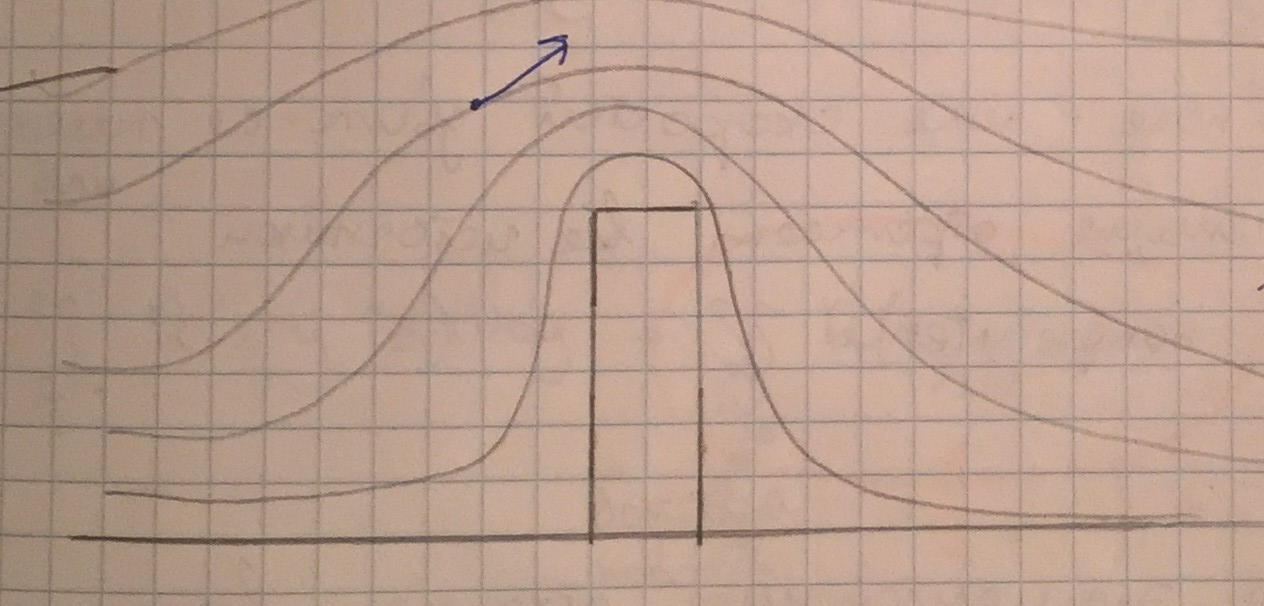
\includegraphics[width = 12cm]{physicalSenseSurface2Kind}

в каждой точке есть направление (аэродинамика, гидродинамика)

\begin{title}[\Large]
  Формула Астроградского - Гаусса
\end{title}

\begin{define}[дивергенции]
  Если в области $D$ заданое дифференцируемое векторное поле $\vec F(x,y,)
  = (P, Q, R)$ то скалярная фукнция (дивергенция)
  $$
  div \vec F = \frac{\partial P}{\partial x} + \frac{\partial Q}{\partial y}
  + \frac{\partial R}{\partial z}
  $$
\end{define}

\begin{theorem}
  Если $\vec F$ непрервыное дифференцируемое векторное поле в области $R^3$
  Тело $T$ в этой области ограниченное кусочно гладкой поверхности $P$
  (дырки разрешаются) $P = \partial T$ тогда
  $$
  \iint_P P dy dz + Q dz dx + R dx dy =
  \iiint_T div \vec F dxdydz
  $$
\end{theorem}

\begin{proof}
  Тело $T$ является эелментарным относительно всех координатных плоскостей
  $$
  T = \{(x, y,z): ~ (x,y) \in D ~~ \varphi(x,y) \le z \le \psi(x,y)\}
  $$
  1)
  $$
  \iiint_T \frac{\partial R}{\partial z} dxdydz = \iint_D dxdy
  \int^{\psi(x,y)}_{\varphi(x,y)} \frac{\partial R}{\partial z} dz =
  $$
  $$
  = \iint_D (R(x,y, \psi(x,y)) - R(x,y, \varphi(x,y))) dx dy =
  $$
  $$
  \iint_{P^+} R(x,y,z) dx dy + \iint_{P^-} R(x,y,z) dxdy + \iint_{P_0}
  R(x,y,z) dxdy
  $$
  Аналогичено

  2)
  $$
  \iiint_T \frac{\partial P}{\partial x} = \iint_P P dydz
  $$
  используя что тело $T$ элементарно относительно плоскости $yOz$

  3)
  $$
  \iiint_T \frac{\partial Q}{\partial y} = \iint_P Q dzdy
  $$
  используя что тело $T$ элементарно относительно плоскости $xOz$

  Далее складываем и получаем формулу Астроградского-Гаусса.

  Распространяется и на случай когда тело $T$ можно разбить на конечное число
  плоскостей элементарных относительно координатных плоскостей.

  В частности таким телов является многогранник.
\end{proof}

\begin{block}[Следствие]
  Формула для вычисления объема, если известна поверхность
  $$
  V(T) = \frac{1}{3} \iint_P xdydz + ydzdx + zdxdy
  $$
  $$
  \iiint_T \left( \frac{\partial P}{\partial x} + \frac{\partial Q}{\partial y}
  + \frac{\partial R}{\partial z} \right) dxdydz = \frac{1}{3} \iiint_T dxdydz =
  \frac{V(T)}{3} ~~~ P = x ~~ Q = y ~~ R = z
  $$
\end{block}

\begin{title}[\Large]
  Соленоидальные поля
\end{title}

\begin{define}[допустивости]
  Поверхность $P$ будем называть допустивой в теле $T \subset R^3$ если
  ограниченная часть пространства данной поверхностью полностью содержится
  (в теле $T$) или граница ограничиваесят в $R^3$

  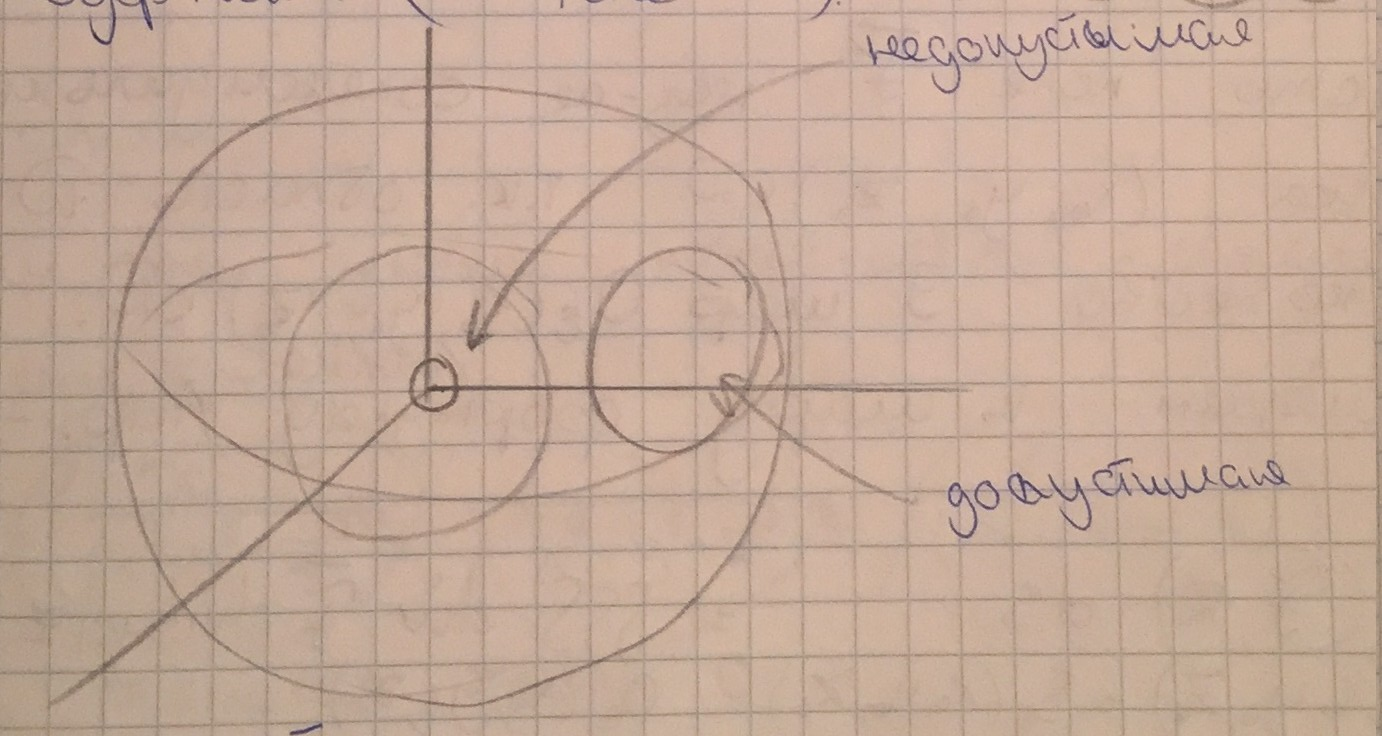
\includegraphics[width = 12cm]{acess}
\end{define}

\begin{define}[соленоидальности]
  Векторное поле $\vec F(x,y,z) \in T$ называется соленоидальным если
  $\forall P \subset T$
  $$
  \iint_P (\vec F, \vec n) ds = \iint_P Pdydz + Q dzdx + R dxdy = 0
  $$
\end{define}

\begin{define}[поверхностно односвязанно]
  Область $D \subset R^3$ называется поверхностно односвязанной если
  $\forall P \subset D$ ограниченная данной поверхностью частью пространства
  также содержится в $D$ (обласить без дырок)
\end{define}

\begin{block}[Критерий соленоидальности поля]
  Для того чтобы векторное поле $\vec F(x,y,z)$ непрерывно дифференцируемое в
  области $D$ было соленоидальным в области $D$ необходимо, а в случае когда
  область $D$ поверхностно односвязанно достаточно, чтобы
  $\forall (x,y,z) \in D ~~ div \vec F = 0$ (сумма частных производных)
\end{block}

\begin{proof}
  $\Leftarrow$ Пусть поле $\vec F$ называется соленоидальным точка
  $(x_0, y_0, z_0) \in D$ так как область $D$ открытое множество то $\exists$
  шар $O_{\varepsilon}(x_0, y_0, z_0) \subset D$

  применим к шару формулу Астроградского-Гаусса
  $$
  \iint_{\partial O_{\varepsilon}(x_0, y_0, z_0) =
  S_{\varepsilon}(x_0, y_0, z_0)} (\vec F, \vec n) ds =
  \iiint_{O_{\varepsilon}} div \vec F dxdydz =
  $$
  $$
  (x_i, y_i, z_i) \subset O_{\varepsilon}(x_0, y_0, z_0) ~~ \text{средняя точка
  лежит где-то в шаре}
  $$
  $$
  = div \vec F(x_0, y_0, z_0) \iiint_{O_{\varepsilon}(x_0, y_0, z_0)} dxdydz =
  div F(x_0, y_0, z_0) \frac{4}{3} \pi \varepsilon^3
  $$
  $\frac{4}{3} \pi \varepsilon^3$ объем шара
  $$
  div \vec F(x_0, y_0, z_0) = \frac{\iint_{S_{\varepsilon}(x_0, y_0, z_0)}
  (\vec F, \vec n) ds}{\frac{4}{3} \pi \varepsilon^3}
  $$
  $$
  \lim_{\varepsilon \to 0} div \vec F(x_0, y_0, z_0) = \lim_{\varepsilon \to 0}
  \frac{\iint_{S_{\varepsilon}(x_0, y_0, z_0)}(\vec F, \vec n) ds}
  {\frac{4}{3} \pi \varepsilon^3} = 0
  $$
  в любой точке области $div$ оказывается равной нулю так как поле соленоидально

  $\Rightarrow$ Пусть $div \vec F = 0 ~~ \forall (x,y,z) \in D$ D - поверхностно
  односвязанно.

  Расмотрим произвольную поверхность $P \subset D$ так как $D$ - поверхность
  односвязанна, то тело $\partial T = P$ ограничена данной поверхностью и
  полностью содержится
  $$
  \iint_P (\vec F, \vec n) ds = \iiint div \vec F dx dy dz = 0
  $$
\end{proof}

\begin{title}[\Large]
  Теорема Стокса
\end{title}

\begin{theorem}[Стокса]
  Пусть $\vec F(x,y,z) = (P,Q,R)$ векторное поле
  $$
  rot \vec F =
  \left|
  \begin{array}{ccc}
    \vec i & \vec j & \vec k \\
    \frac{\partial}{\partial x} &
    \frac{\partial}{\partial y} &
    \frac{\partial}{\partial z} \\
    P & G & R
  \end{array}
  \right| =
  \left(
    \frac{\partial R}{\partial x}
    -
    \frac{\partial Q}{\partial z},
    \frac{\partial R}{\partial z}
    -
    \frac{\partial P}{\partial x},
    \frac{\partial Q}{\partial x}
    -
    \frac{\partial P}{\partial y},
  \right) = ~ \text{ротор} ~ \vec F
  $$
  степень закругленности (вихрь)

  $T \subset R^3 ~~ \Gamma \subset T$ контур (замкнутая кривая) края
  поверхности $P$ то есть $\Gamma = \partial P$

  $\vec \varphi = \vec \varphi(u, \upsilon) ~~~ (u, \upsilon) \in [D]$
  отображение $R^2 \to R^3$

  $\gamma = \partial D$ ориентированна положительно
  $$
  \left\{
  \begin{array}{l}
    u = u(t) \\
    \upsilon = \upsilon(t)
  \end{array}
  \right. ~~ t \in [a,b]
  $$
  тогда $\Gamma = \vec \varphi(\gamma)$ тоже ориентированна.

  Сторона которая содержится $\vec n$ называется согласованной с ориентацией
  $\gamma$
\end{theorem}

\begin{theorem}
  Пусть поле $\vec F$ непрерывно дифференцируем в некоторой области $R^3$ в
  которой задана простая почти проставя поверхность $P$ с параметрическим
  заданием $\vec \varphi = \vec \varphi(u, \upsilon)$ а $(u, \upsilon \in [D]$
  бегает в замыкани $D$

  Если $\Gamma = \partial P$ (край поверхности P) ориентация которого
  согласованна с выбором стороы поверхности $P$ то
  $$
  \int_{\Gamma} (\vec F, d\vec \varphi) = \iint_P (rot \vec F, \vec n) ds
  $$
  $$
  \int_{\Gamma} Pdx + Qdy + Rdz =
  $$
  $$
  = \iint_P
  \left(
    \frac{\partial R}{\partial y}
    -
    \frac{\partial Q}{\partial z}
  \right) dy dz
  +
  \left(
    \frac{\partial P}{\partial z}
    -
    \frac{\partial R}{\partial x}
  \right) dz dx
  +
  \left(
    \frac{\partial Q}{\partial x}
    -
    \frac{\partial P}{\partial y}
  \right) dx dy
  $$
  обобщение формулы Грина
\end{theorem}

\begin{proof}
  $$
  \int_{\Gamma} P dx = \iint_P
    \frac{\partial P}{\partial z} dz dx
    -
    \frac{\partial P}{\partial y} dx dy
  $$
  $$
  \int_{\Gamma} P dx = \iint_{\gamma}
    P
    \left(
      \frac{\partial x}{\partial u} du
      +
      \frac{\partial x}{\partial \upsilon} d\upsilon
    \right)
  =
  $$
  $$
  \int_{\gamma} Pdx + Qdy = \iint_D
    \left(
      \frac{\partial Q}{\partial x}
      -
      \frac{\partial Q}{\partial x}
    \right)
    dx dy
  $$
  $$
  = \iint_{[D]}
    \left[
      \left(
        \frac{\partial P}{\partial x}
        \frac{\partial x}{\partial u}
        +
        \frac{\partial P}{\partial y}
        \frac{\partial y}{\partial u}
        +
        \frac{\partial P}{\partial z}
        \frac{\partial z}{\partial u}
      \right)
      \frac{\partial x}{\partial \upsilon}
      +
      P \frac{\partial^2 x}{\partial u \partial \upsilon}
    \right.
    -
  $$
  $$
    \left.
      -
      \left(
        \frac{\partial P}{\partial x}
        \frac{\partial x}{\partial \upsilon}
        +
        \frac{\partial P}{\partial y}
        \frac{\partial y}{\partial \upsilon}
        +
        \frac{\partial P}{\partial z}
        \frac{\partial z}{\partial \upsilon}
      \right)
      \frac{\partial x}{\partial u}
      -
      P \frac{\partial^2 x}{\partial \upsilon \partial u}
    \right]
    du d\upsilon
  =
  $$
  $$
  = \iint_{[D]}
    \left[
      \frac{\partial P}{\partial z}
      \left(
        \frac{\partial z}{\partial x}
        \frac{\partial u}{\partial \upsilon}
        -
        \frac{\partial z}{\partial x}
        \frac{\partial \upsilon}{\partial u}
      \right)
      -
      \frac{\partial P}{\partial y}
      \left(
        \frac{\partial y}{\partial x}
        \frac{\partial \upsilon}{\partial u}
        -
        \frac{\partial y}{\partial x}
        \frac{\partial u}{\partial \upsilon}
      \right)
    \right]
    du d\upsilon =
  $$
  $$
  = \iint_P
    \frac{\partial P}{\partial z} dz dx
    -
    \frac{\partial P}{\partial y} dx dy
  $$
\end{proof}

\begin{title}[\Large]
  Потенциальные векторные поля в $R^3$
\end{title}

\begin{define}[потенциального векторного поля]
  Непрерывное векторное поле $\vec F(x,y,z) = (P, Q, R)$ называется
  потенциальным в какой-то области $D \subset R^3$ $u = u(x,y,)$ если
  выполняется равенство
  $$
  \grad (u) = \vec F ~~ \Leftrightarrow ~~
  \left\{
  \begin{array}{l}
    \frac{\partial u}{\partial x} = P \\
    \frac{\partial u}{\partial y} = Q \\
    \frac{\partial u}{\partial z} = R
  \end{array}
  \right.
  $$
\end{define}

\begin{theorem}
  Пусть $\vec F$ непрерывное векторное поле в области $D$ следующие 3 условия
  эквивалентны

  1)
  $$
  \int_{L \subset D} Pdx + Qdy + Rdz = 0
  $$
  2)
  $$
  \int_{L_{ABCD}} Pdx + Qdy + Rdz = 0
  $$
  не зависит от вида ломанной $L_{AB}$, а зависит только от граничных точек

  3)
  $\vec F = (P, Q, R)$ является потенциальным в $D$
\end{theorem}

\begin{define}[линейной односвязонности]
  Область $D \subset R^3$ называется линейно односвязаной если $\forall$
  замкнутой кусочно-гладкой кривой $\Gamma \subset D$ $\exists$ поверхность
  $P \subset D$ такая что $\Gamma = \partial P$
\end{define}

\begin{block}[Критерий потенциальности поля]
  Для того чтобы непрерывно дифференцируемое векторное поле $\vec F = (P, Q, R)$
  была потенциально необходимо, а в случае, когда область $D$ линейно
  односвязанна достаточно $\forall (x,y,z) \in D ~~ rot \vec F(x,y,z) = \vec 0$
\end{block}

\begin{proof}
  $\Rightarrow$ Пусть $\vec F$ потенциально
  $$
  u = u(x,y,z) ~~~
  \left\{
  \begin{array}{l}
    \frac{\partial u}{\partial x} = P \\
    \frac{\partial u}{\partial y} = Q \\
    \frac{\partial u}{\partial z} = R
  \end{array}
  \right.
  $$
  $$
  \frac{\partial R}{\partial y}
  =
  \frac{\partial^2 u}{\partial y \partial z}
  ~~~
  \frac{\partial Q}{\partial z}
  =
  \frac{\partial^2 u}{\partial z \partial y}
  $$
  $$
  \left(
    \frac{\partial R}{\partial y}
    -
    \frac{\partial Q}{\partial z}
    ,
    \frac{\partial P}{\partial z}
    -
    \frac{\partial R}{\partial x}
    ,
    \frac{\partial Q}{\partial x}
    -
    \frac{\partial P}{\partial y}
  \right)
  = rot \vec F
  ~~~
  \Rightarrow (0, 0, 0) = rot \vec F
  $$

  $\Leftarrow$ Пусть $rot \vec F = \vec 0$

  Берем замкнутую ломанную $L \in D ~~~ P \subset D ~~~ \exists L = \partial P$
  $$
  \int_L (\vec F, d \vec \varphi) = \iint_P (rot \vec F, \vec n) ds = 0
  $$
  так как область линейно односвязанна. Из теоремы 1 поле потенциально
\end{proof}
